\documentclass[runningheads,a4paper]{llncs}

\usepackage{amssymb}
\setcounter{tocdepth}{3}
\usepackage{graphicx}

\usepackage{url}

\usepackage{graphicx}
% \usepackage{caption}
% \usepackage{subcaption}
\usepackage[caption=false]{subfig}

\begin{document}

\mainmatter

\title{Automatic Perspective Correction of Manuscript Images}

\author{Ryan Baumann\inst{1} \and Christopher Blackwell\inst{2} \and W. Brent Seales\inst{1}}

\institute{University of Kentucky
\and
Furman University}

\maketitle

\section{Introduction}

Frequently, images of rare documents must be taken under strict time constraints, 
when a chance opportunity arises, and with equipment that is less than ideally suited 
for precise digitization. This can often result in uncalibrated images
whose contents are nonetheless qualitatively useful. Due to the logistics of document
imaging, perspective distortion is a common artifact which can manifest itself in
images taken under these constrained circumstances. We propose an automated approach for
correcting this perspective distortion, even for uncalibrated images of documents
with irregular page edges containing no regular text.

\section{Background}

Details about imaging here.

\section{Related Work}

Numerous work exists for performing document perspective correction by exploiting the presence of
common text features, such as linear text baselines in printed texts.
As a result, many of these techniques need to be tweaked depending upon morphological features of
the written language of the document in question.
However, for our documents,
many pages had no such features, consisting only of handwritten text and physical plant
specimens. As a result, our approach is fairly unique in that it uses only physical page boundaries to
perform the perspective correction. An advantage to this is that it can handle “blank” pages or pages
consisting only of images or haphazard writing. In addition, because the manuscript pages we are dealing with have
cockled, uneven edges, our boundary detection needs to be relatively robust to the “noise” of these uneven edges.

\section{Perspective Correction Algorithm}

The perspective correction algorithm functions by applying a few steps in sequence:

\begin{figure}[htbm]
  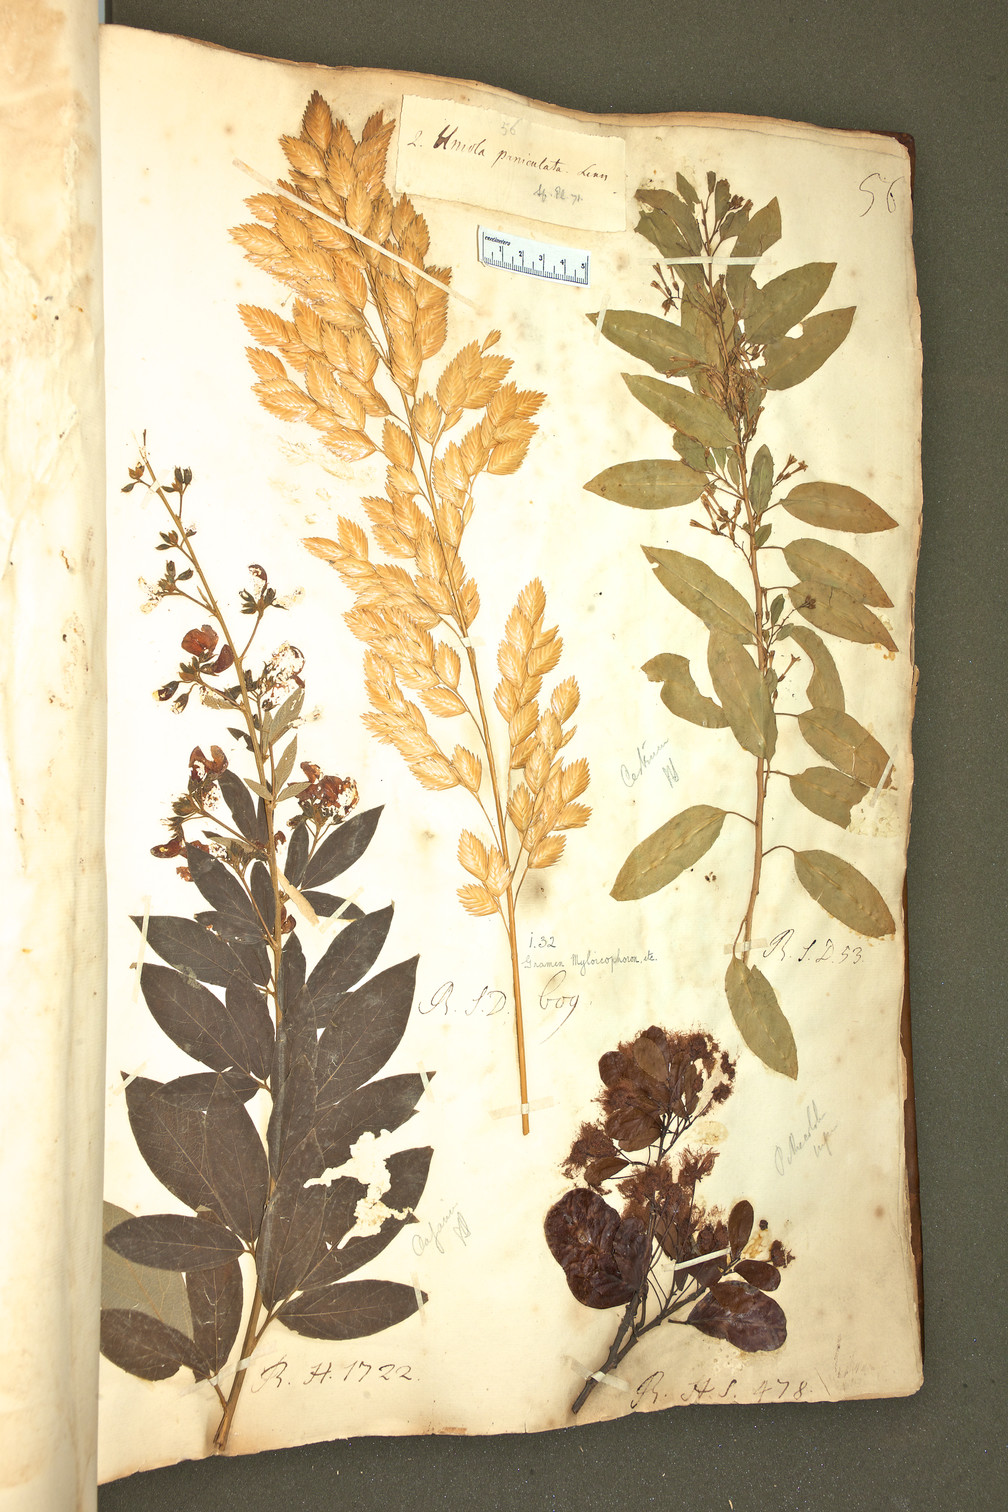
\includegraphics[width=\textwidth]{figures/original.jpg}
  \caption{Original image}\label{fig:original}
\end{figure}

\begin{figure}[htbm]
  \subfloat[Masked image]{
    
\includegraphics[width=.48\textwidth]{figures/Catesby_HS232_056_0602-masked.jpg}
    \label{fig:masked}
  }
  \subfloat[Canny edge lines]{
    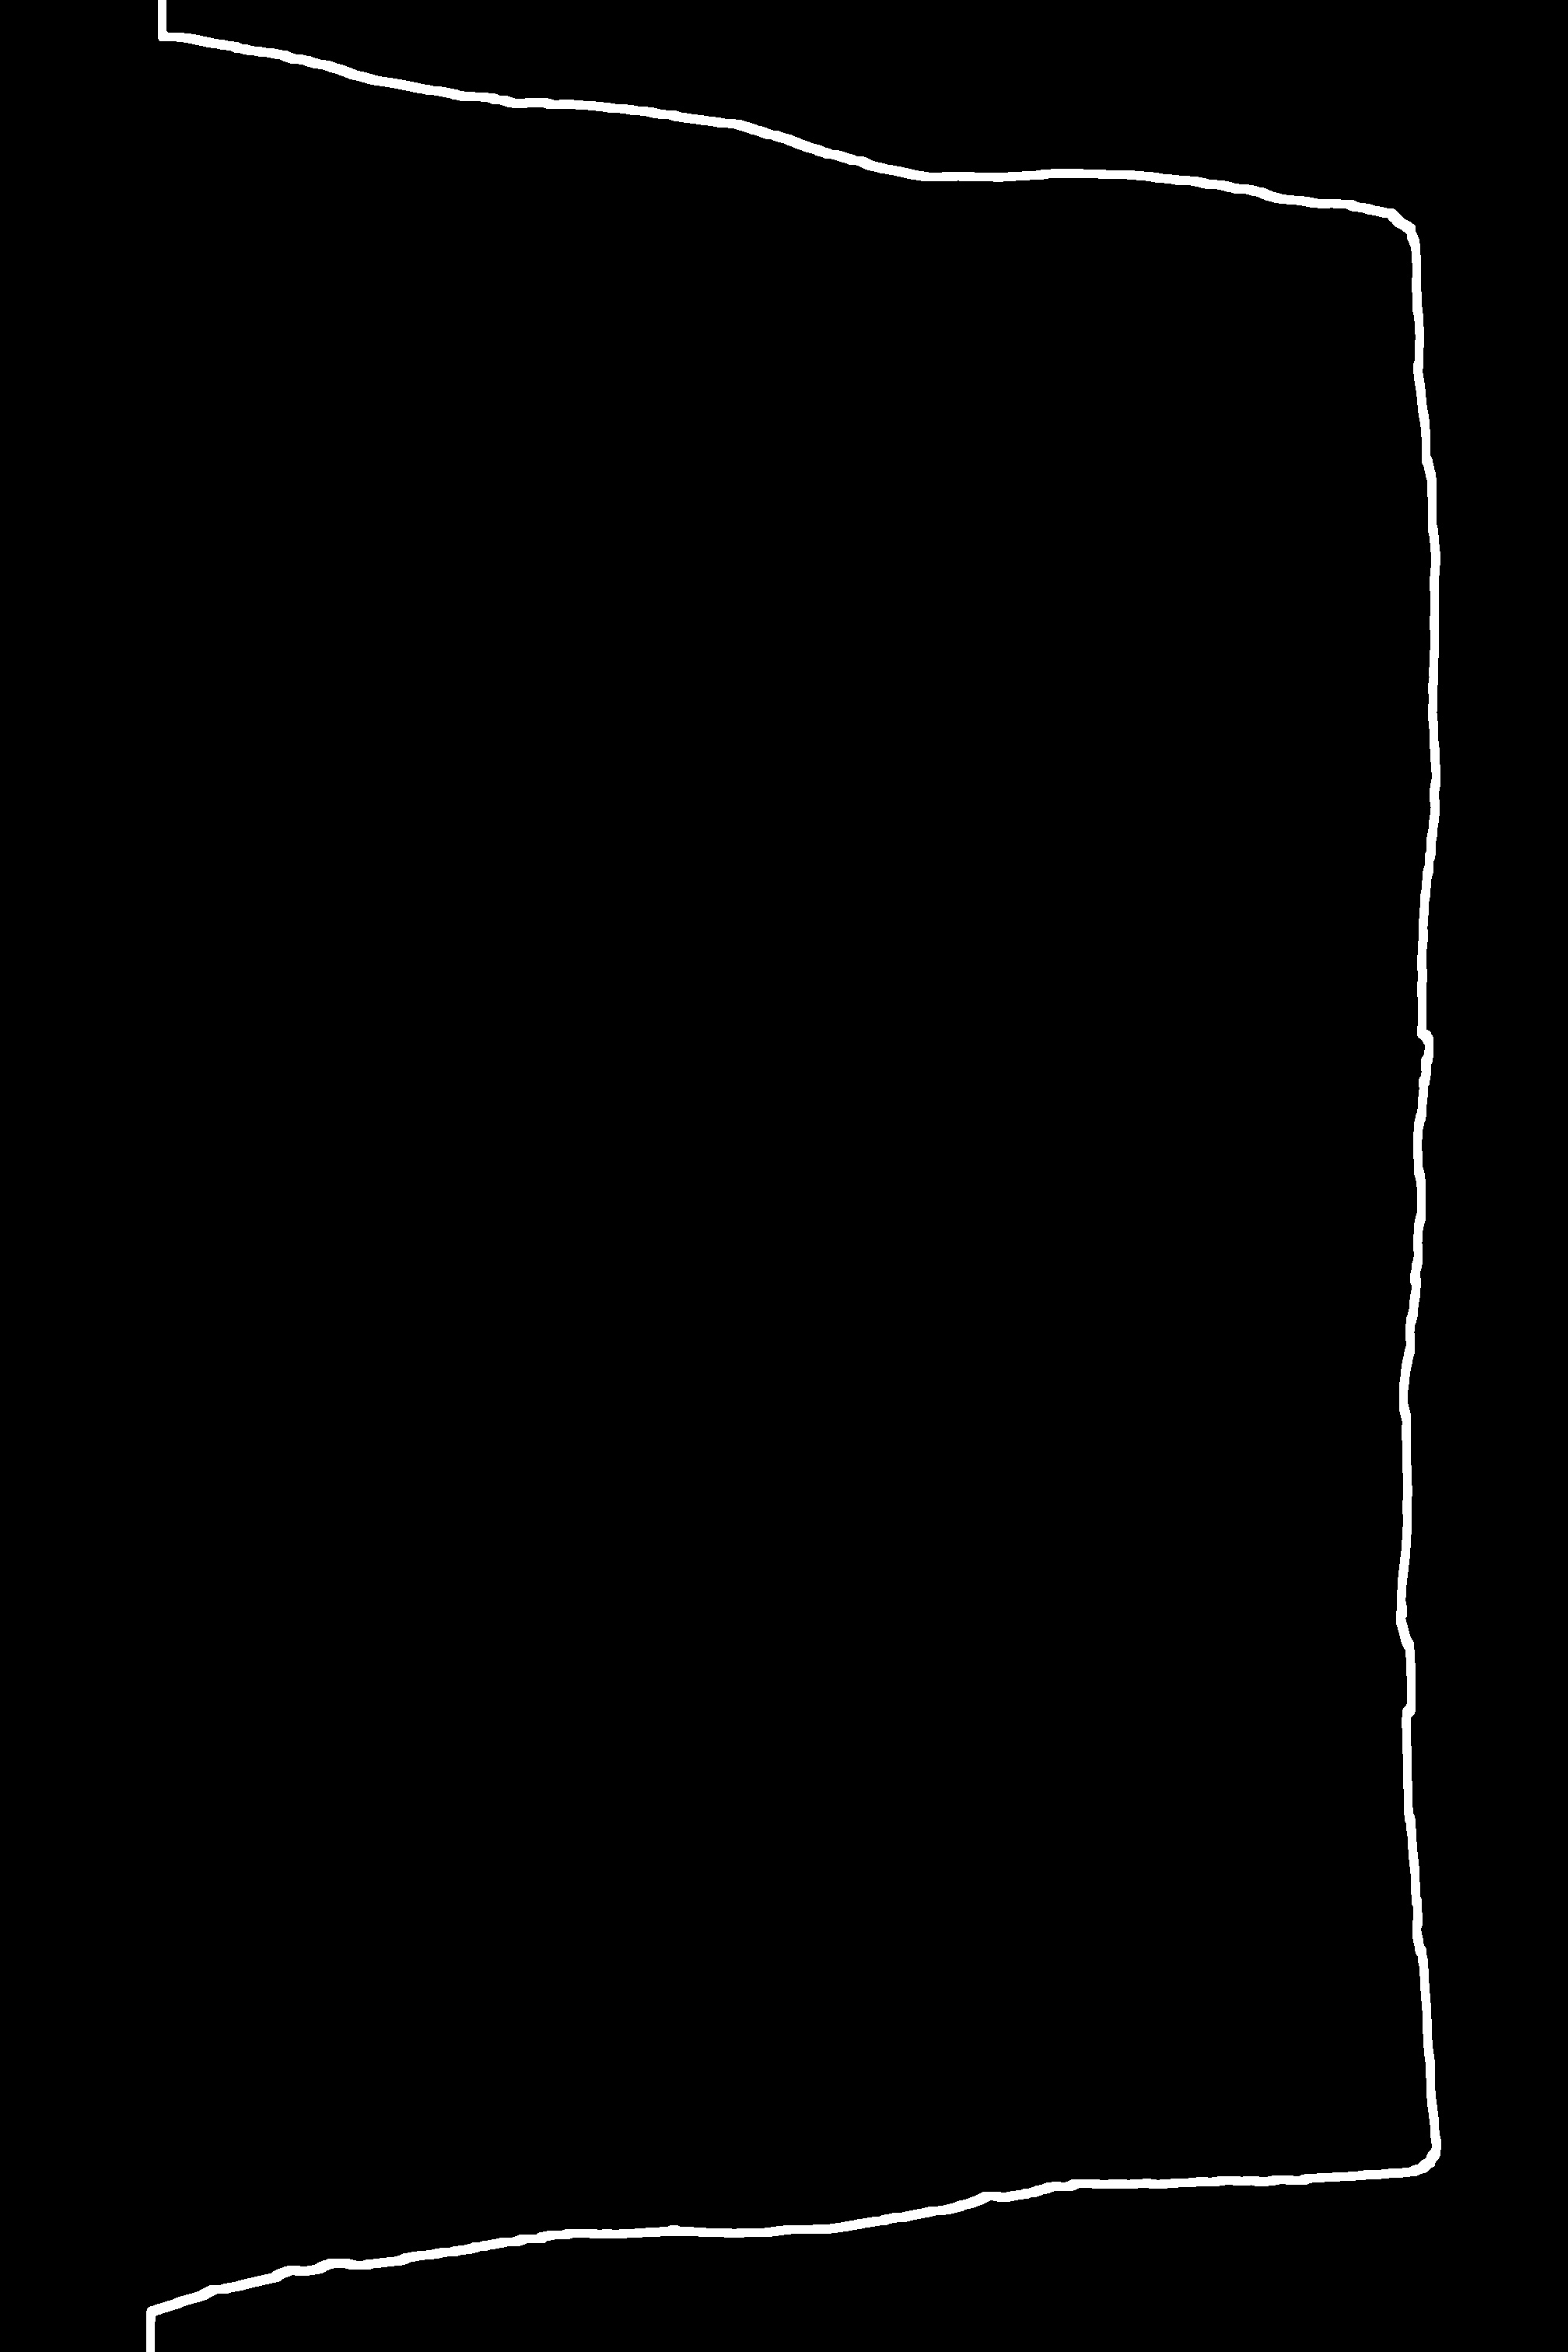
\includegraphics[width=.48\textwidth]{figures/Catesby_HS232_056_0602-canny.jpg}
    \label{fig:canny}
  }

  \subfloat[Hough line detection]{
    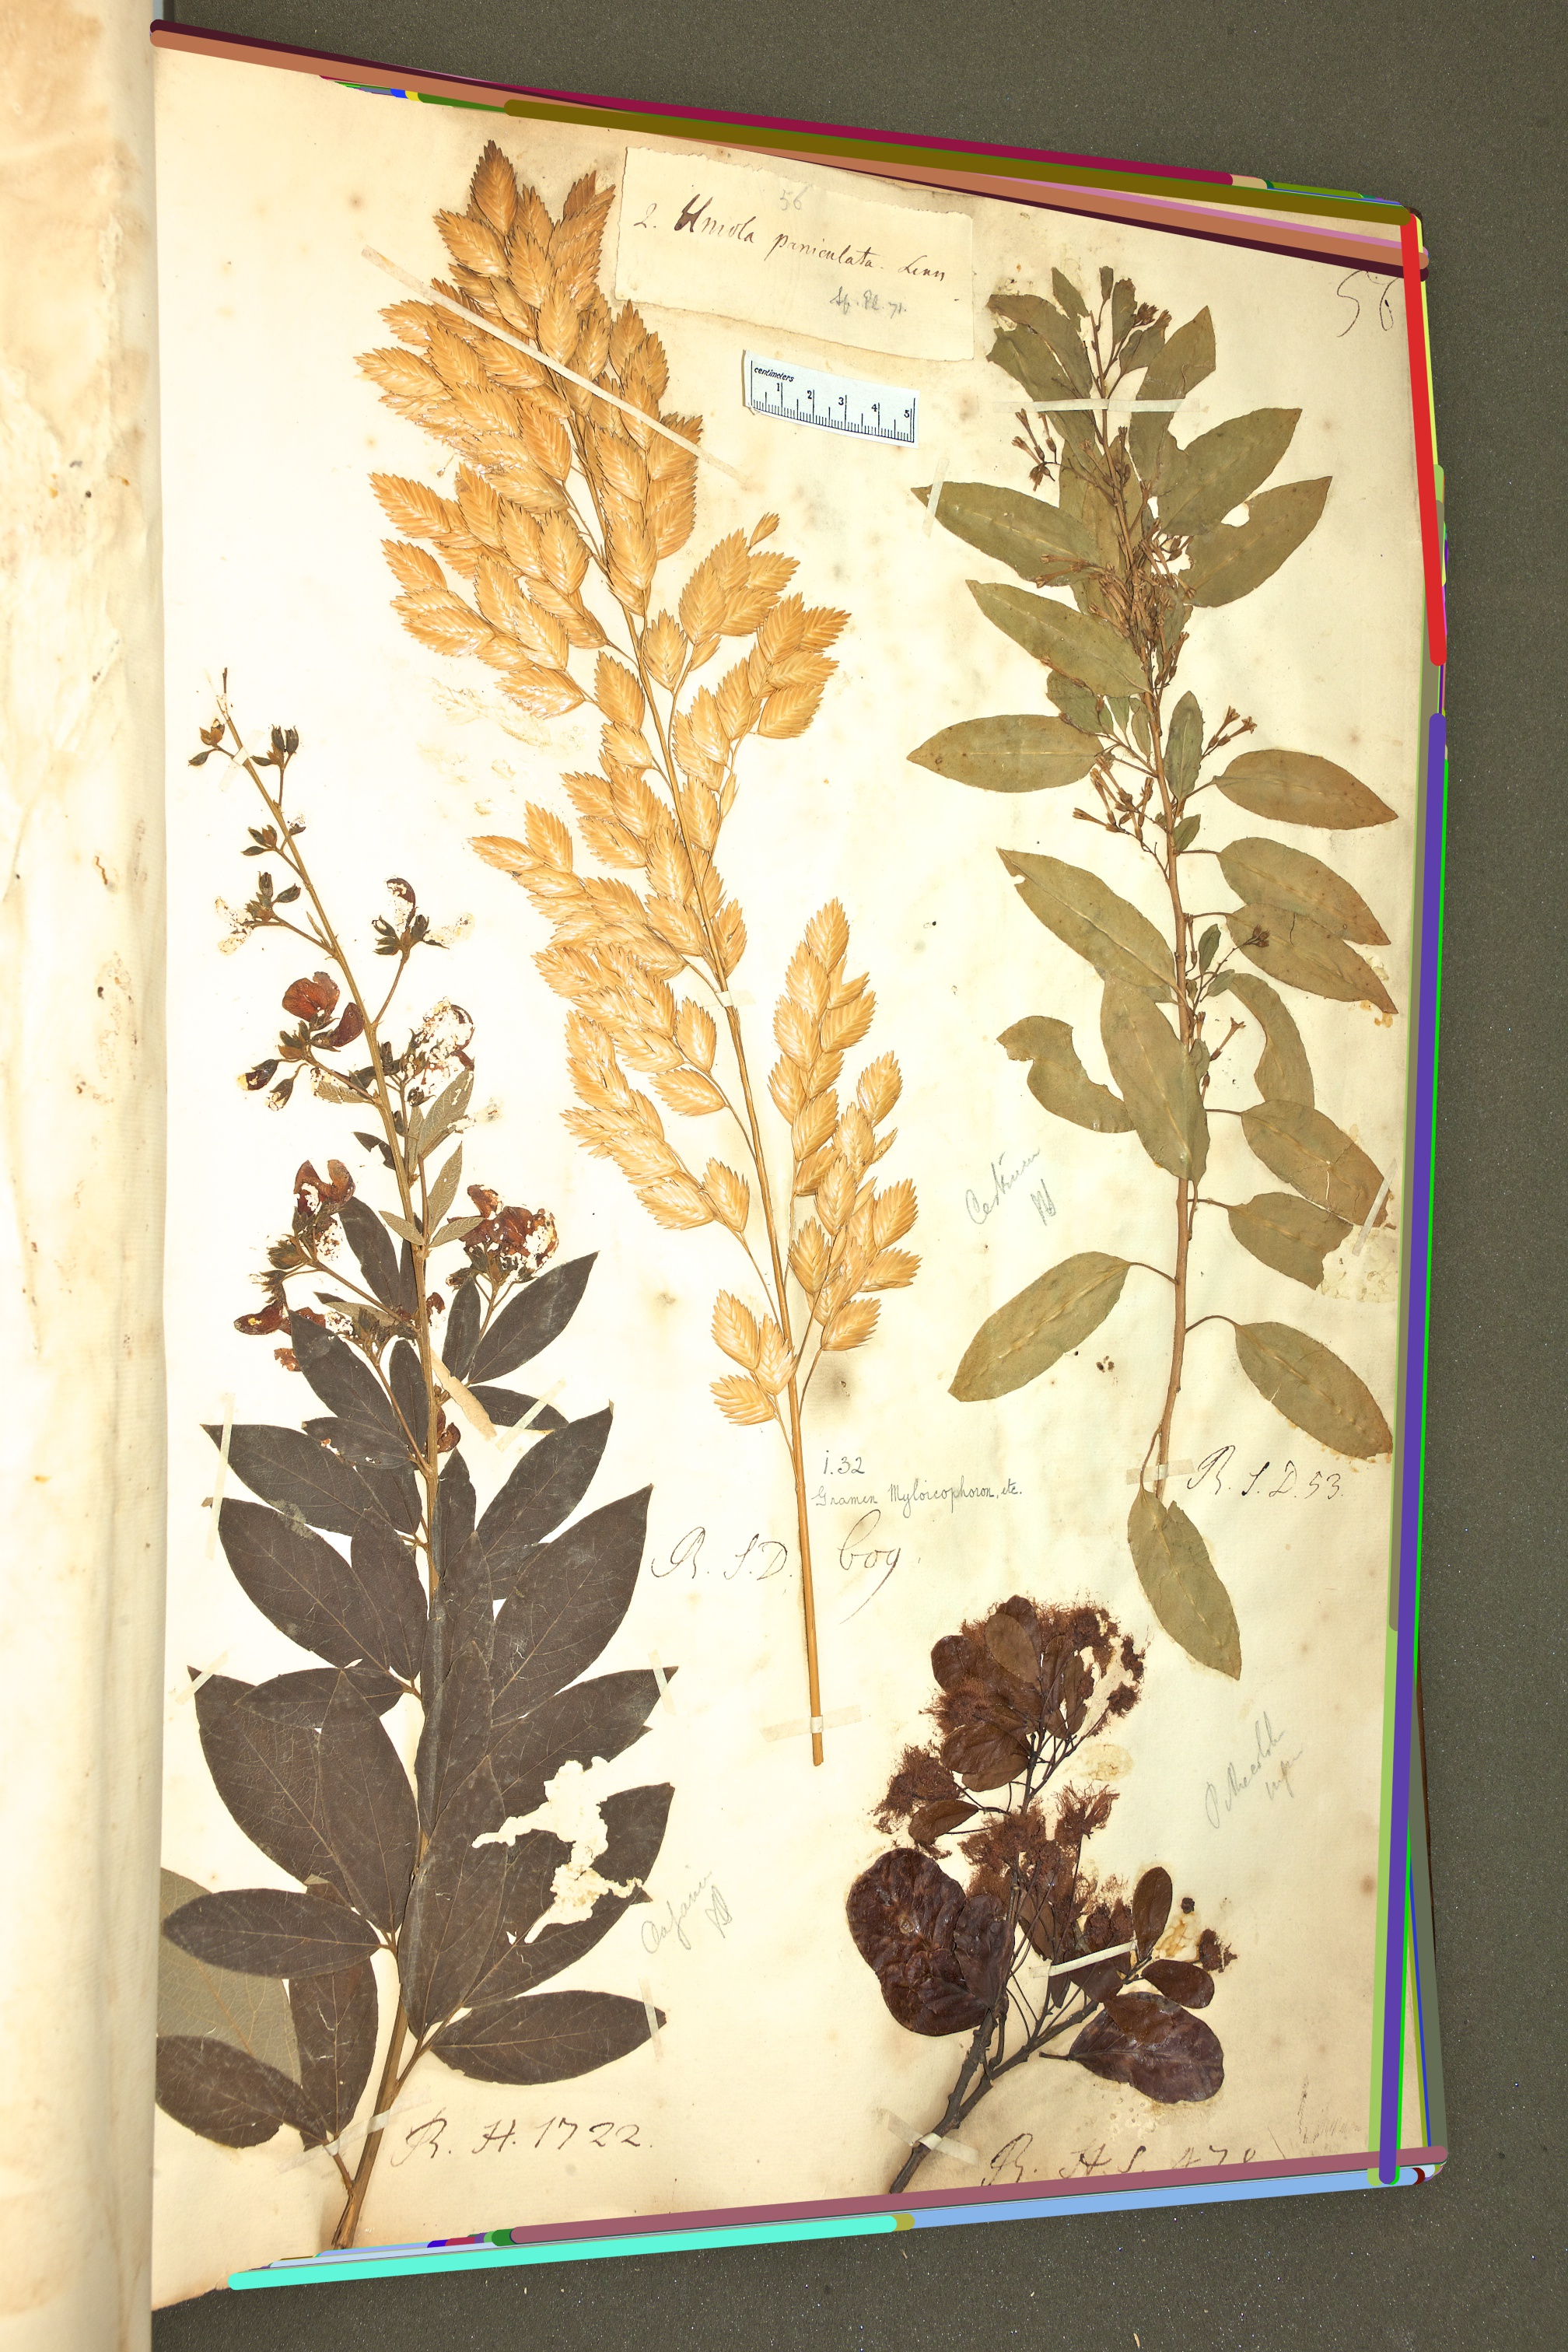
\includegraphics[width=.48\textwidth]{figures/Catesby_HS232_056_0602-hough.jpg}
    \label{fig:hough}
  }
  \subfloat[Classified lines]{
    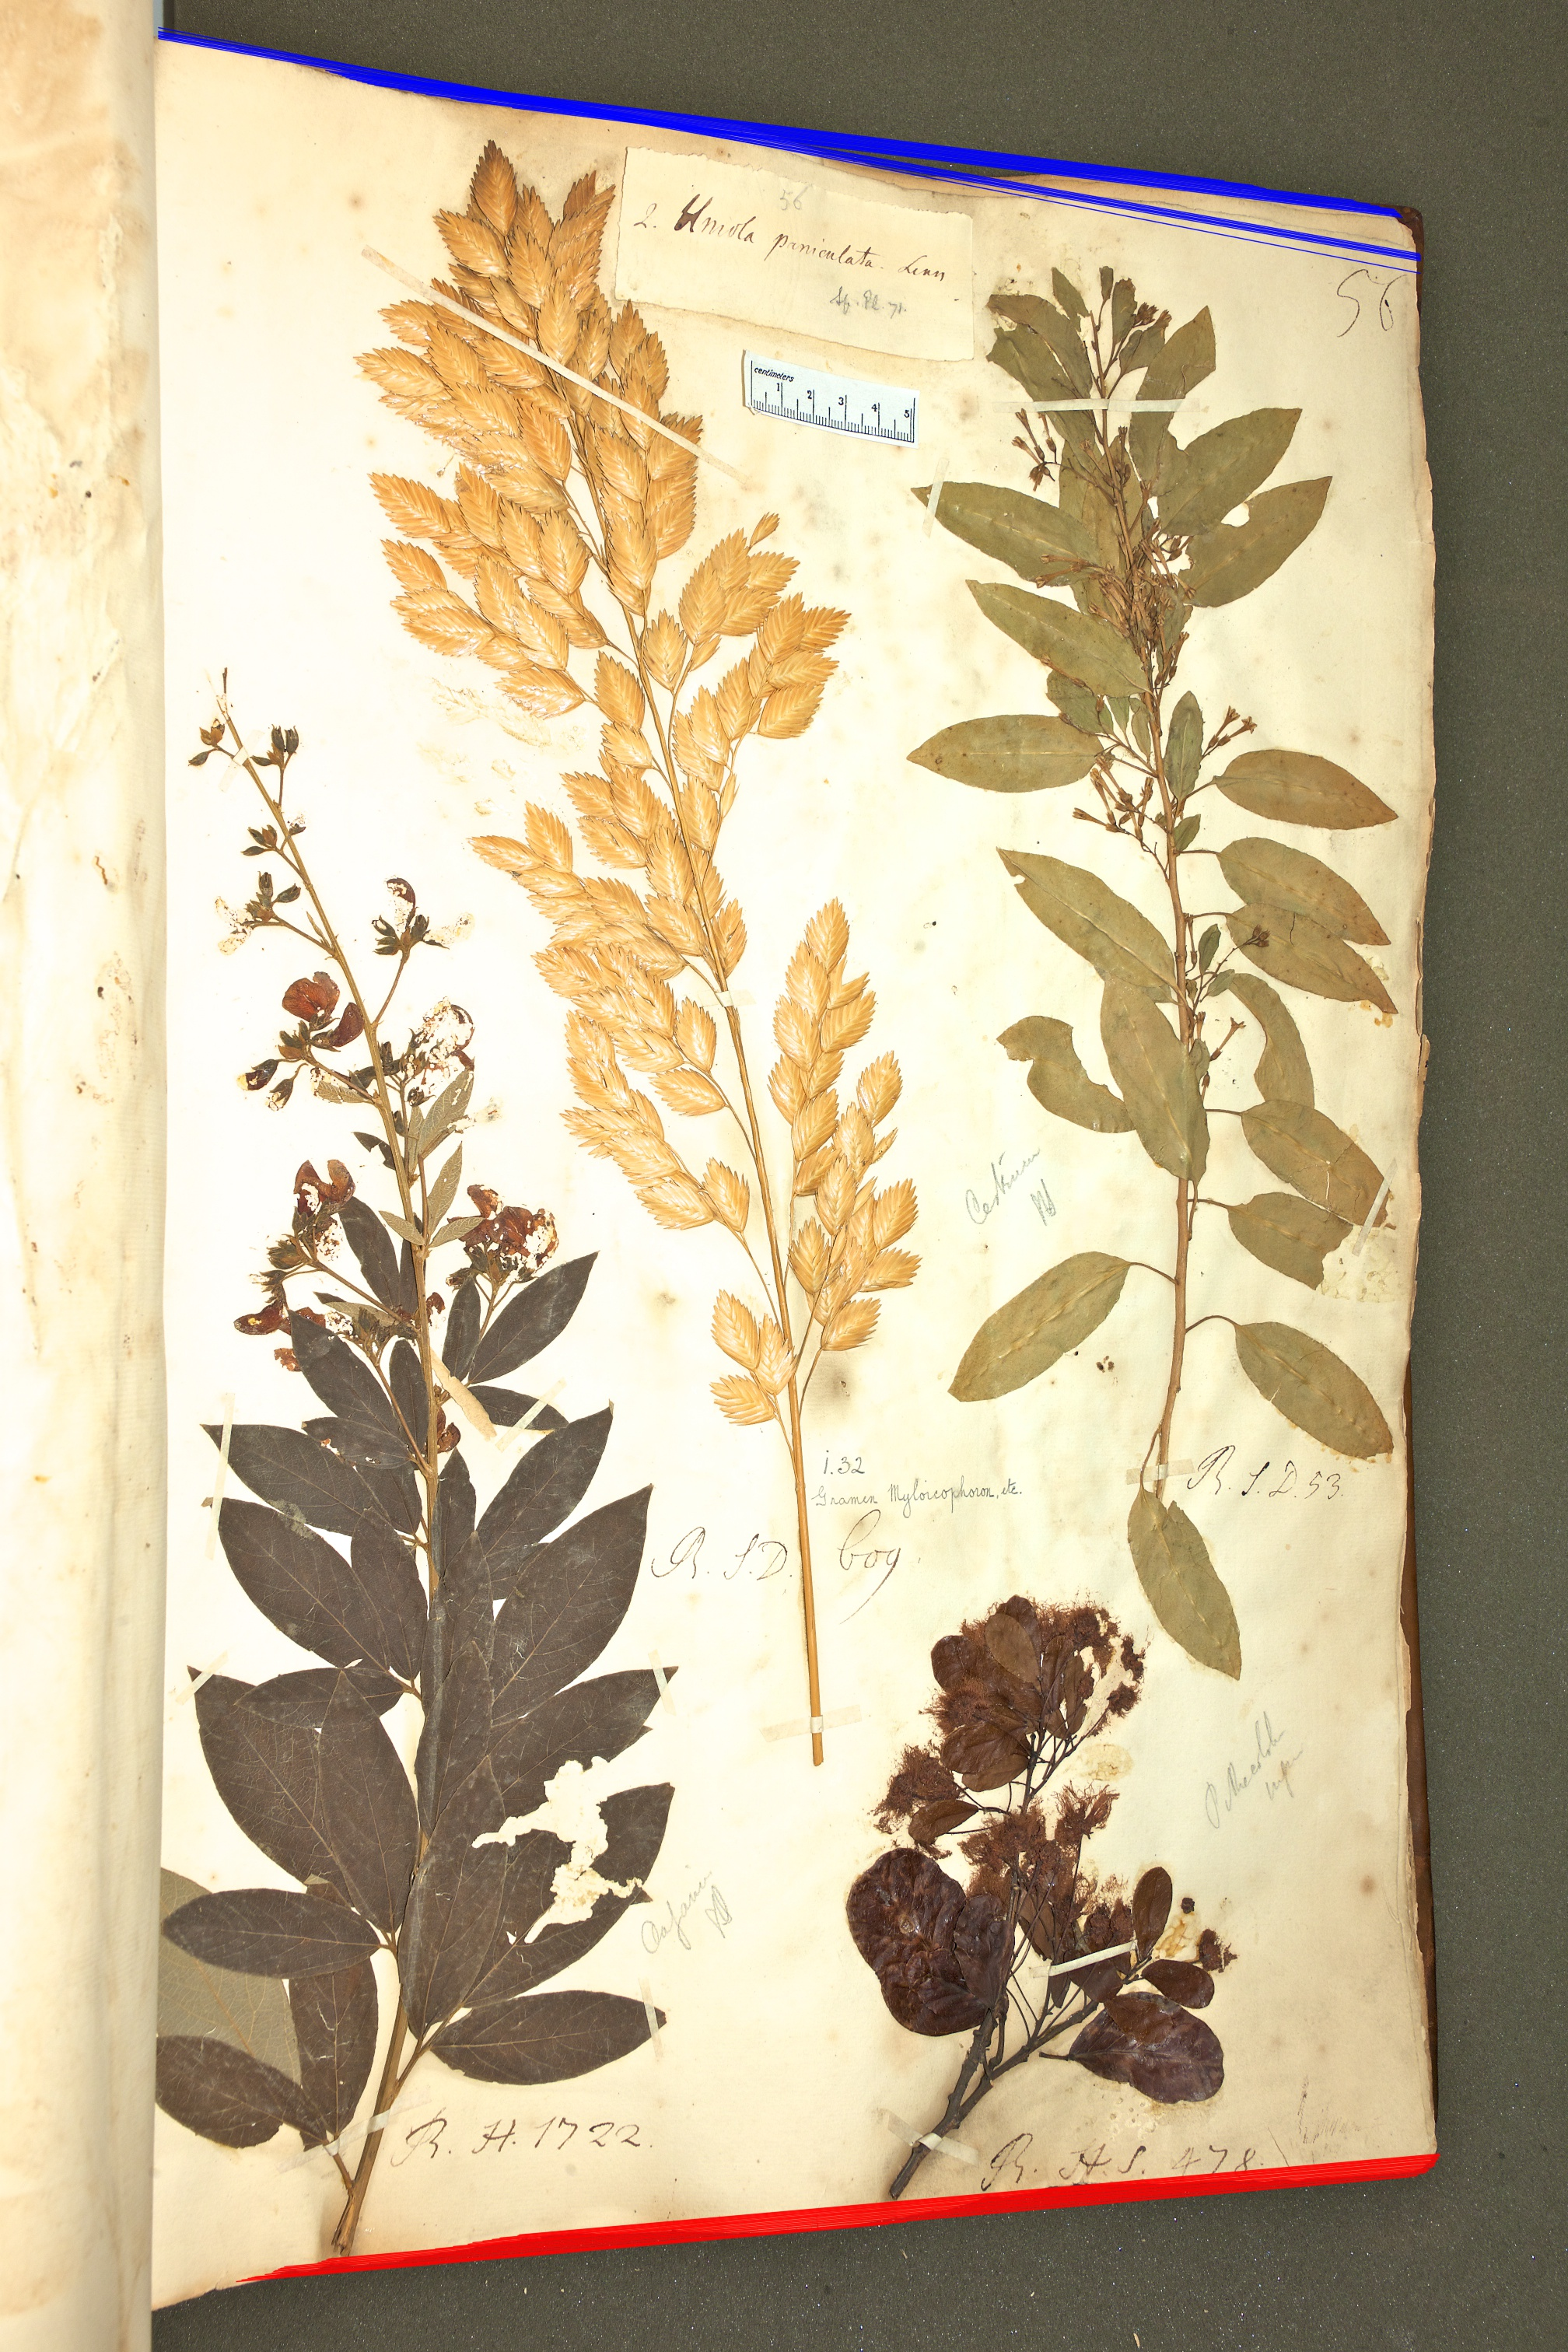
\includegraphics[width=.48\textwidth]{figures/Catesby_HS232_056_0602-hough-classified.jpg}
    \label{fig:classified}
  }
  \caption{Pre-processing steps}\label{fig:processing}
\end{figure}

\begin{figure}[htbm]
  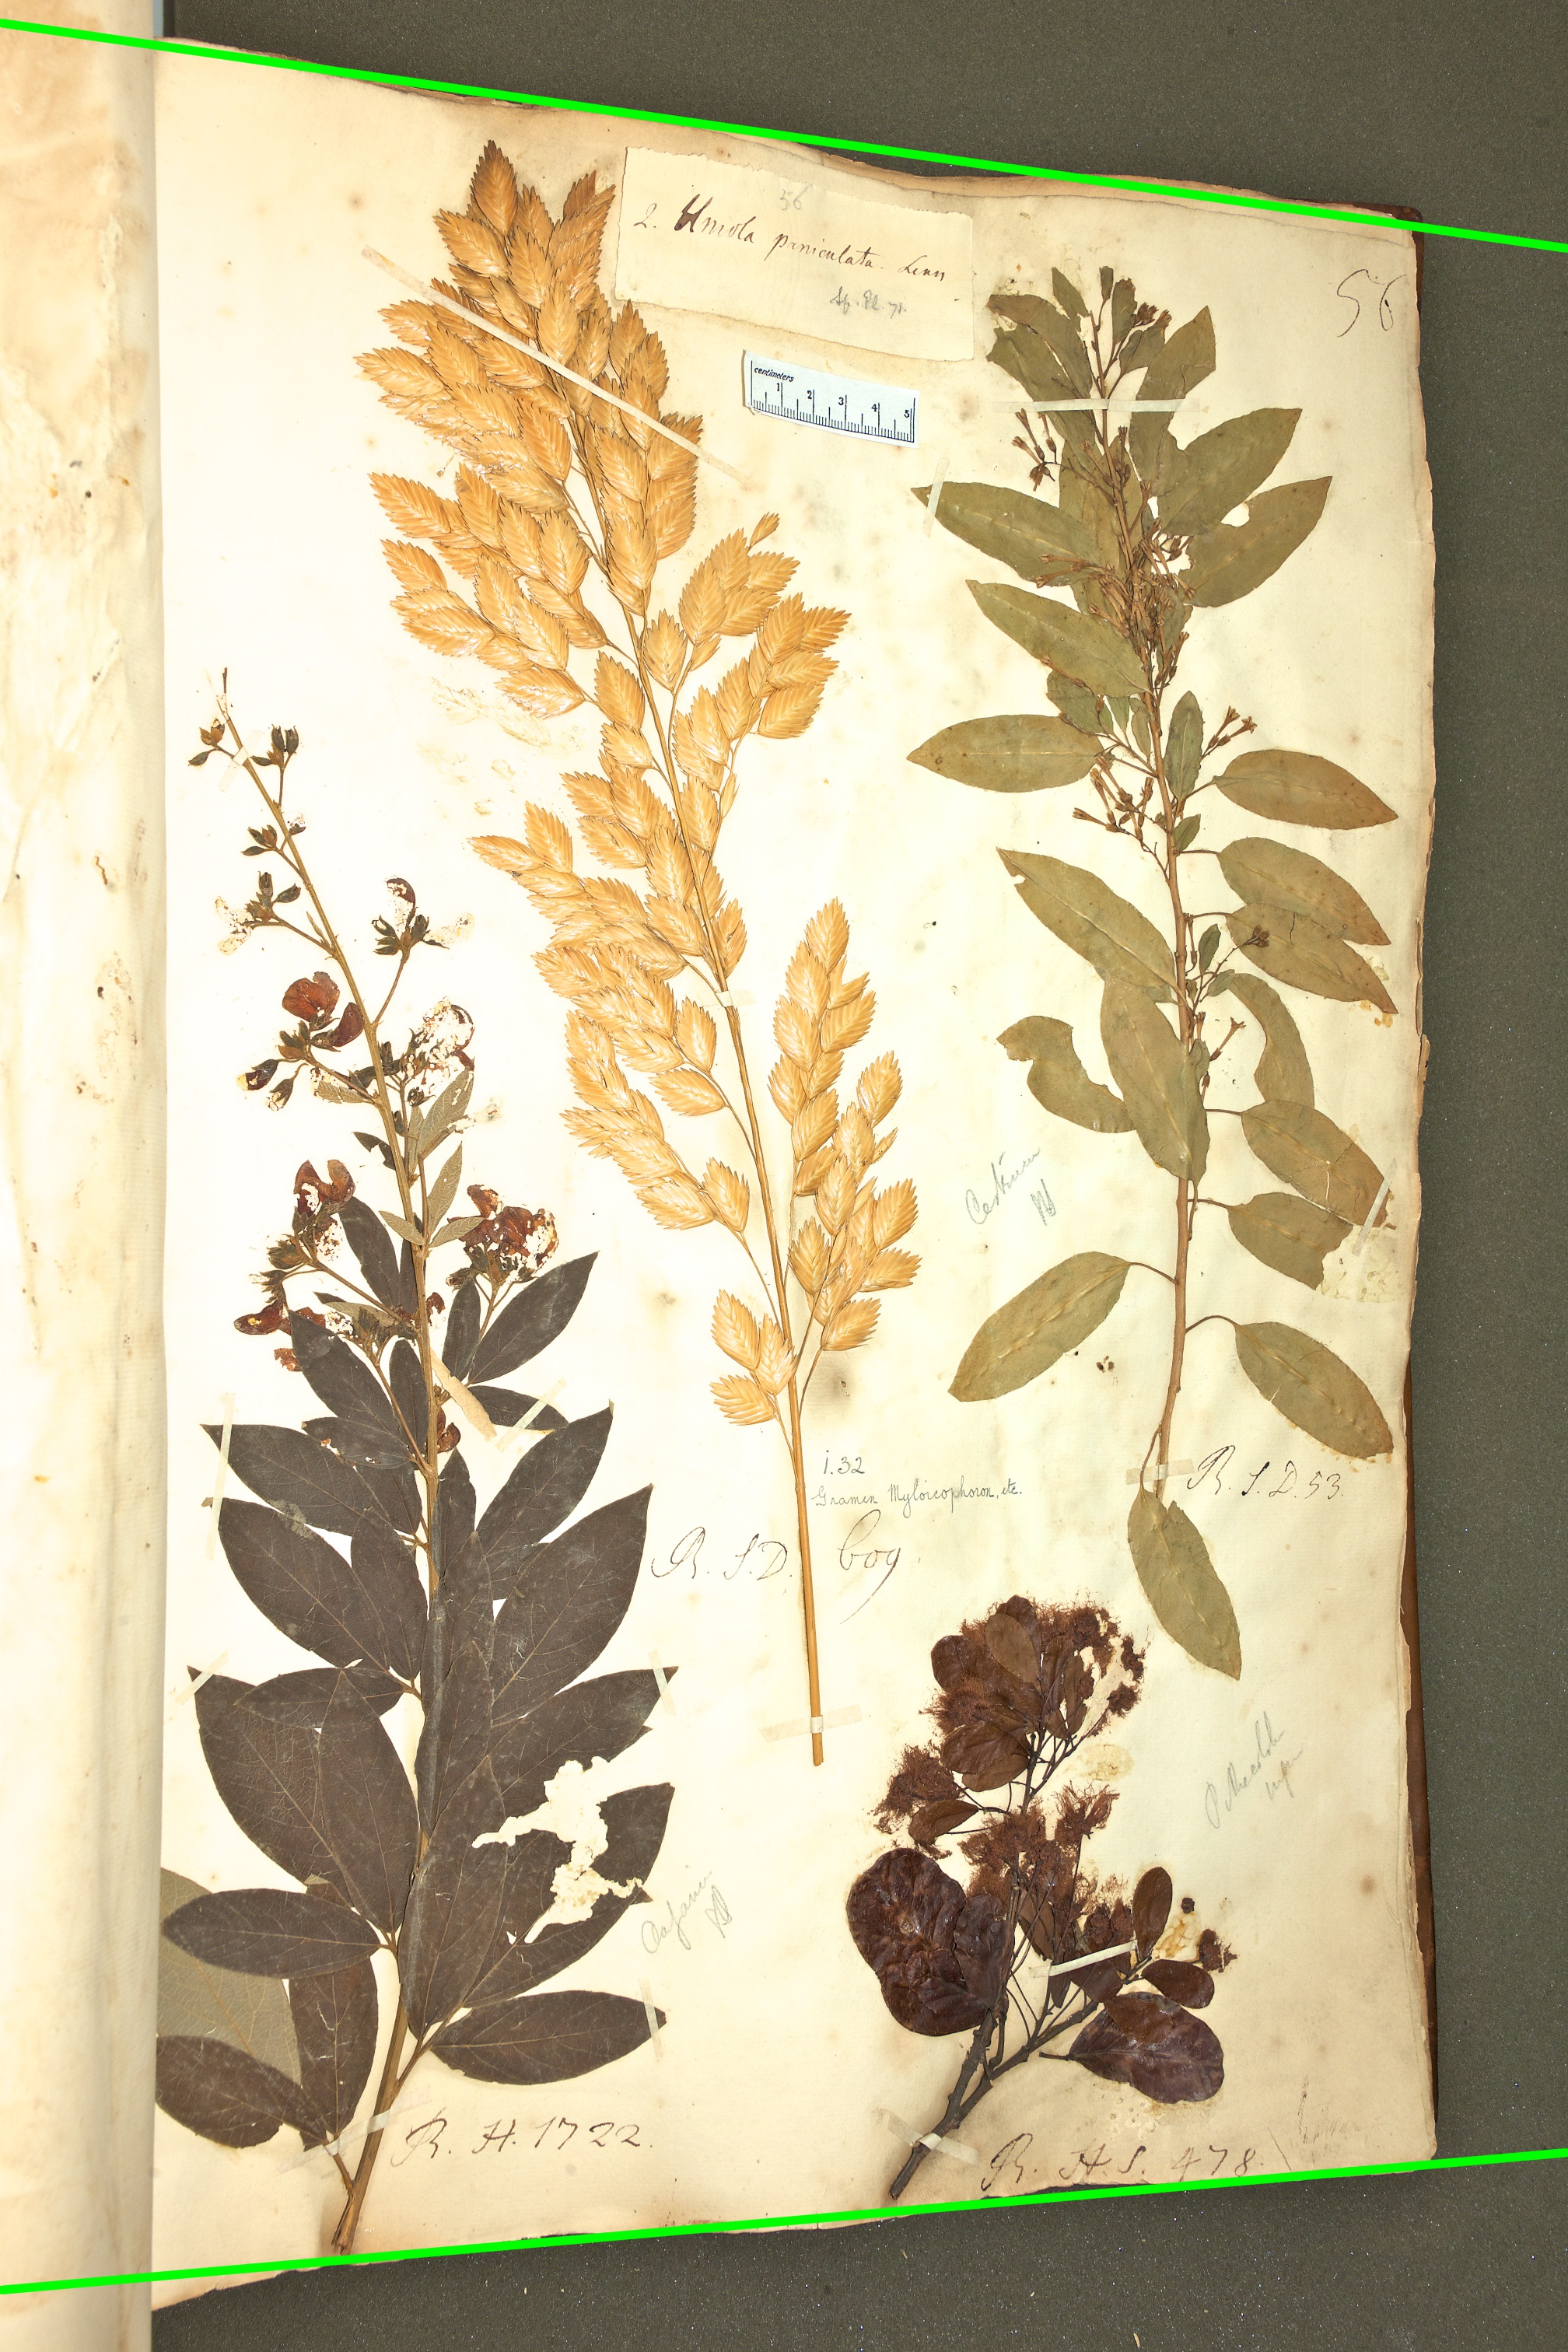
\includegraphics[width=\textwidth]{figures/Catesby_HS232_056_0602-hough-averaged.jpg}
  \caption{Averaged lines}\label{fig:averaged}
\end{figure}

\begin{figure}[htbm]
  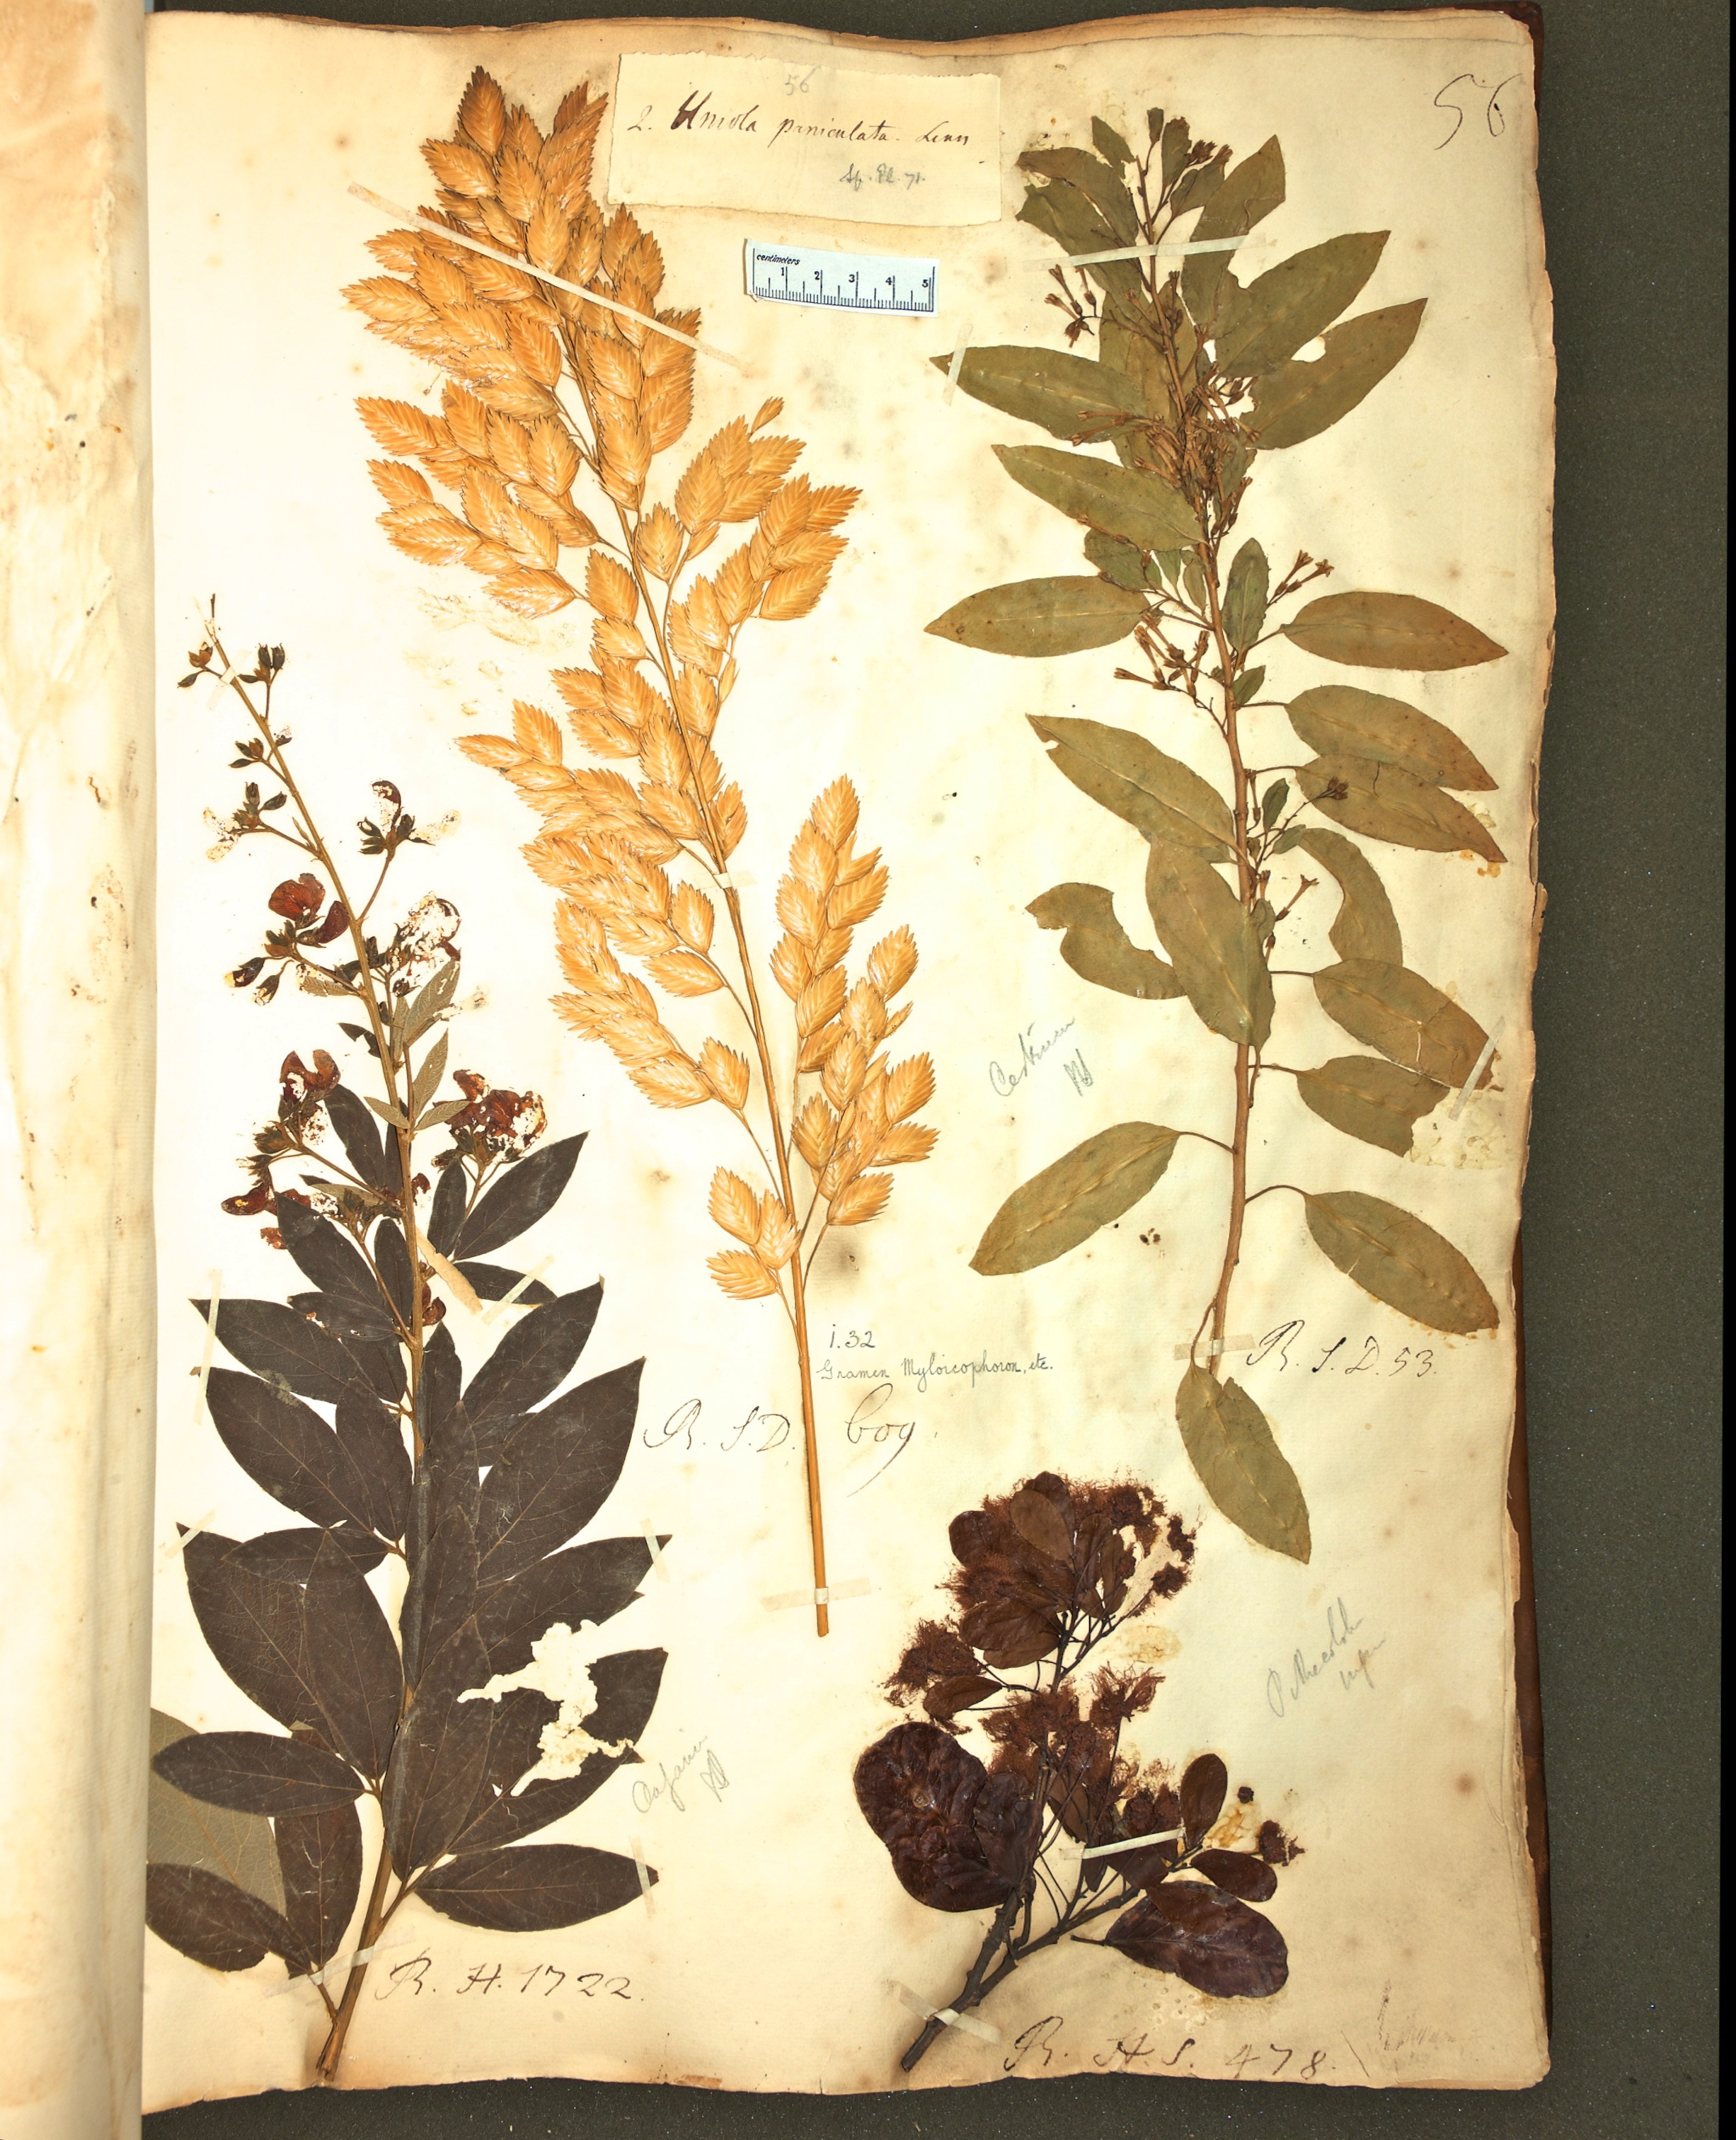
\includegraphics[width=\textwidth]{figures/Catesby_HS232_056_0602-unwarped-stretch.jpg}
  \caption{Unwarped image}\label{fig:unwarped}
\end{figure}

\begin{enumerate}
  \item Foreground/background segmentation. (Figure \ref{fig:masked})
  \item Canny edge detection followed by dilation to turn the mask image into a line image. (Figure \ref{fig:canny})
  \item Hough line detection to detect lines. (Figure \ref{fig:hough})
  \item Line classification to classify the detected lines as “top” or “bottom” page edge lines. (Figure \ref{fig:classified})
  \item Line averaging to find the “average” line for the top and bottom edge lines. (Figure \ref{fig:averaged})
  \item Compute homography for transforming the slanted top and bottom page lines into straight lines.
  \item Application of the resulting perspective warp. (Figure \ref{fig:unwarped})
\end{enumerate}

For our images, most were made with a fairly consistent backdrop, so the foreground/background segmentation operates by performing a flood fill on the corners of a gaussian-smoothed version of the image. This exploits the assumption that the page will not fill the full image all the way around, as in such a case, our perspective correction would likely be unable to accurately detect all the page edges which it uses to compute homography. We then remove blobs whose area is less then half the image, as we assume the page still makes up most of the image. 

This gives us a mask image as seen in figure (figure ref here). Since we want to use Hough line detection, we first need to transform the mask edges into lines, which we do using a Canny edge detector and dilation, the results of which can be seen in figure (figure ref here).

We can then perform Hough line detection, using a probabilistic Hough transform which gives us line segments for every line detected in the image. We classify these lines as belonging to either the “top” or “bottom” of the page by seeing which half of the image height the start and end points are in, and restricting it to only lines with a $\pm 45\,^{\circ}$ angle. This also filters out edges detected along the left and right side of the page.

We can then average these lines to get the average “line” for the top and bottom page edges. We extend these lines to the image edges, and construct a quadrilateral matrix using them for the top and bottom. We then compute a destination quadrilateral matrix using the assumption that the top edge should be “brought up” to the highest point to form a straight line (while maintaining line length), and similarly for the bottom edge being brought down, forming a rectangle. We can then use these two quads to compute a perspective transform which will warp our source quadrilateral into our destination rectangle. We then apply the resulting perspective warp to the whole image, resulting in a dewarped image.

\section{Results}

\section{Conclusions and Future Work}

\section{Acknowledgments}

\bibliographystyle{splncs}
\bibliography{icadl12}

\end{document}
